\documentclass[tikz,border=2pt]{standalone}
\usepackage{tikz}

\begin{document}
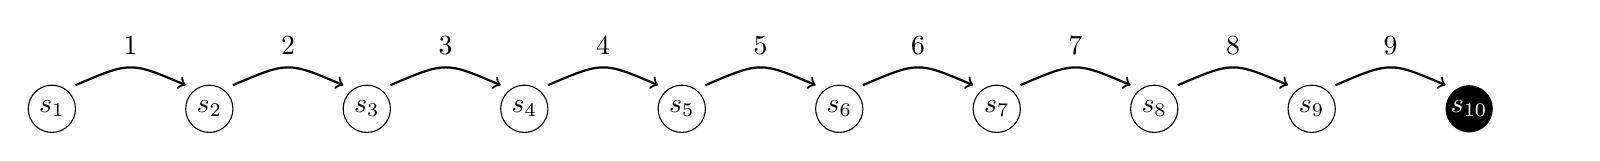
\begin{tikzpicture}[scale=2.0]

\def\r{0.15};
\def\n{10};
\foreach \x in {\n}{
       \fill[fill=black] (\x, 0) circle [radius=\r];
       \node[white] at (\x, 0) {$s_{\x}$};
}
\foreach \x in {1,...,9}{
       \draw (\x, 0) circle [radius=\r];
       \node[black] at (\x, 0) {$s_{\x}$};
}
\fill[fill=white] (\n+0.5, 0) circle [radius=\r];
\foreach \x/\t in {1/1,2/2,3/3,4/4,5/5,6/6,7/7,8/8,9/9}{
       \draw [black, thick, ->] (\x+\r, \r) .. controls (\x+0.5, 0.3) .. (\x+1-\r, \r);
       \node[black] at (\x+0.5, 0.4) {\t};
       }

\end{tikzpicture}
\end{document}
